\documentclass[12pt]{scrartcl}
\usepackage{amsmath,amssymb,amsfonts,mathrsfs}
\usepackage{miller}
\usepackage{multirow}
\usepackage{subeqnarray}
\usepackage{bm}
\usepackage{natbib}

\usepackage{graphicx}
\graphicspath{{./}{./figure/}{../Figures/}}
\DeclareGraphicsExtensions{.pdf,.png}
\usepackage[pdftex,                                     % hyper-references for pdftex
bookmarksnumbered=true,%                                % generate bookmarks with numbers
%pagebackref=true,%                                      % generate backref in biblio
colorlinks=true,%
linkcolor=blue,
citecolor=red,
urlcolor=blue,
pdfpagelabels=false,
plainpages = false,
]{hyperref}%

\usepackage[capitalise]{cleveref}                                   % for clever referencing


\usepackage{tikz}
\usetikzlibrary{shapes.geometric, arrows}
\usetikzlibrary{automata,positioning}


% SOMETHING USEFUL
\newcommand{\ie}{\textit{i.e.}}
\newcommand{\eg}{\textit{e.g.}}
\newcommand{\cf}{\textit{cf.}}
\newcommand{\Euler}{\term{Euler}}
\newcommand{\Gauss}{\term{Gauss}}
\newcommand{\Fourier}{\term{Fourier}}

\newcommand{\kB}{\ensuremath{k_\text{B}}}

% FUNCTIONS AND OPERATORS
\newcommand{\transpose}[1]{\ensuremath{{#1}^{\text T}}}
\newcommand{\inverse}[1]{\ensuremath{{#1}^{-1}}}
\newcommand{\invtranspose}[1]{\ensuremath{{#1}^{\text{-T}}}}
\newcommand{\sign}[1]{\ensuremath{\operatorname{sgn}\left({#1}\right)}}
\newcommand{\grad}[1][]{\ensuremath{\operatorname{grad}{#1}}}
\newcommand{\Grad}[1][]{\ensuremath{\operatorname{Grad}{#1}}}
\newcommand{\divergence}[1][]{\ensuremath{\operatorname{div}{#1}}}
\newcommand{\Divergence}[1][]{\ensuremath{\operatorname{Div}{#1}}}
\newcommand{\curl}[1][]{\ensuremath{\operatorname{curl}{#1}}}
\newcommand{\Curl}[1][]{\ensuremath{\operatorname{Curl}{#1}}}
\newcommand{\totalder}[2]{\ensuremath{\frac{\inc{#1}}{\inc{#2}}}}
\newcommand{\partialder}[2]{\ensuremath{\frac{\partial{#1}}{\partial{#2}}}}
\newcommand{\inc}[1]{\ensuremath{\text d{#1}}}
\newcommand{\abs}[1]{\ensuremath{\left|{#1}\right|}}
\newcommand{\norm}[2][]{\ensuremath{\left|\left|{#2}\right|\right|\if\relax\detokenize{#1}\relax\else _{#1}\fi}}
\newcommand{\avg}[1]{\ensuremath{\overline{#1}}}
\newcommand{\fluct}[1]{\ensuremath{\widetilde{#1}}}
\newcommand{\FT}[1]{\ensuremath{\mathcal F\left[{#1}\right]}}
\newcommand{\invFT}[1]{\ensuremath{\mathcal F^{-1}\left[{#1}\right]}}

\newcommand{\domain}[1]{\ensuremath{\mathcal{#1}}}
\newcommand{\tnsrfour}[1]{\ensuremath{\mathbb{#1}}}
\newcommand{\tnsr}[1]{\ensuremath{\mathbf{#1}}}
\newcommand{\tnsrgreek}[1]{\ensuremath{\bm{#1}}}
\newcommand{\vctr}[1]{\ensuremath{\mathbf{#1}}}
\newcommand{\vctrgreek}[1]{\ensuremath{\bm{#1}}}

% SPECIAL TENSORS
\newcommand{\eyetwo}{\ensuremath{\tnsr I}}
\newcommand{\eyefour}{\ensuremath{\tnsrfour I}}

% VARIABLES
\newcommand{\defmap}{\ensuremath{\vctrgreek{\chi}}}
\newcommand{\stiffness}{\tnsrfour C}
\newcommand{\fPK}{\ensuremath{\tnsr P}}
\newcommand{\fPKcomponent}{\ensuremath{P}}
\newcommand{\fPKavg}{\ensuremath{\avg{\fPK}}}
\newcommand{\sPK}{\ensuremath{\tnsr S}}
\newcommand{\F}[1][]{\ensuremath{\tnsr F^{#1}}}
\newcommand{\Fcomponent}[1][]{\ensuremath{F^{#1}}}
\newcommand{\Fdot}[1][]{\ensuremath{\dot{\tnsr F}^{#1}}}
\newcommand{\E}{\tnsr E}
\newcommand{\GL}{\ensuremath{\tnsr E_\text{e}}}
\newcommand{\Favg}{\ensuremath{\avg{\F}}}
\newcommand{\Ffluct}{\ensuremath{\fluct{\F}}}
\newcommand{\Fp}[1][]{\ensuremath{\tnsr F_\text{p}^{#1}}}
\newcommand{\Fpdot}[1][]{\ensuremath{\dot{\tnsr F}_\text{p}^{#1}}}
\newcommand{\Fe}[1][]{\ensuremath{\tnsr F_\text{e}^{#1}}}
\newcommand{\velgrad}{\ensuremath{\tnsr L}}
\newcommand{\Lp}{\ensuremath{\tnsr L_\text{p}}}
\newcommand{\bcFdot}{\ensuremath{\dot{\tnsr F}_\text{BC}}}
\newcommand{\bcF}{\ensuremath{{\F}_\text{BC}}}
\newcommand{\bcfPK}{\ensuremath{{\fPK}_\text{BC}}}
\newcommand{\Burgers}[1]{\ensuremath{\vctr b^{#1}}}
\newcommand{\n}[1]{\ensuremath{\vctr n^{#1}}}
\newcommand{\velocity}[2]{\ensuremath{v^{#1}_\text{#2}}}
\newcommand{\galpha}{\ensuremath{\gamma^{\alpha}}}
\newcommand{\dotgalpha}{\ensuremath{\dot{\gamma}^{\alpha}}}
\newcommand{\cs}{\ensuremath{\tnsrgreek \sigma}}

\newif\ifcuboidshade
\newif\ifcuboidemphedge

\tikzset{
  cuboid/.is family,
  cuboid,
  shiftx/.initial=0,
  shifty/.initial=0,
  dimx/.initial=3,
  dimy/.initial=3,
  dimz/.initial=3,
  scale/.initial=1,
  densityx/.initial=1,
  densityy/.initial=1,
  densityz/.initial=1,
  rotation/.initial=0,
  anglex/.initial=0,
  angley/.initial=90,
  anglez/.initial=225,
  scalex/.initial=1,
  scaley/.initial=1,
  scalez/.initial=0.5,
  front/.style={draw=black,fill=white},
  top/.style={draw=black,fill=white},
  right/.style={draw=black,fill=white},
  shade/.is if=cuboidshade,
  shadecolordark/.initial=black,
  shadecolorlight/.initial=white,
  shadeopacity/.initial=0.15,
  shadesamples/.initial=16,
  emphedge/.is if=cuboidemphedge,
  emphstyle/.style={thick},
}


% TIKZ extension
\newcommand{\tikzcuboidkey}[1]{\pgfkeysvalueof{/tikz/cuboid/#1}}

% Commands
\newcommand{\tikzcuboid}[1]{
    \tikzset{cuboid,#1} % Process Keys passed to command
  \pgfmathsetlengthmacro{\vectorxx}{\tikzcuboidkey{scalex}*cos(\tikzcuboidkey{anglex})*28.452756}
  \pgfmathsetlengthmacro{\vectorxy}{\tikzcuboidkey{scalex}*sin(\tikzcuboidkey{anglex})*28.452756}
  \pgfmathsetlengthmacro{\vectoryx}{\tikzcuboidkey{scaley}*cos(\tikzcuboidkey{angley})*28.452756}
  \pgfmathsetlengthmacro{\vectoryy}{\tikzcuboidkey{scaley}*sin(\tikzcuboidkey{angley})*28.452756}
  \pgfmathsetlengthmacro{\vectorzx}{\tikzcuboidkey{scalez}*cos(\tikzcuboidkey{anglez})*28.452756}
  \pgfmathsetlengthmacro{\vectorzy}{\tikzcuboidkey{scalez}*sin(\tikzcuboidkey{anglez})*28.452756}
  \begin{scope}[xshift=\tikzcuboidkey{shiftx}, yshift=\tikzcuboidkey{shifty}, scale=\tikzcuboidkey{scale}, rotate=\tikzcuboidkey{rotation}, x={(\vectorxx,\vectorxy)}, y={(\vectoryx,\vectoryy)}, z={(\vectorzx,\vectorzy)}]
    \pgfmathsetmacro{\steppingx}{1/\tikzcuboidkey{densityx}}
  \pgfmathsetmacro{\steppingy}{1/\tikzcuboidkey{densityy}}
  \pgfmathsetmacro{\steppingz}{1/\tikzcuboidkey{densityz}}
  \newcommand{\dimx}{\tikzcuboidkey{dimx}}
  \newcommand{\dimy}{\tikzcuboidkey{dimy}}
  \newcommand{\dimz}{\tikzcuboidkey{dimz}}
  \pgfmathsetmacro{\secondx}{2*\steppingx}
  \pgfmathsetmacro{\secondy}{2*\steppingy}
  \pgfmathsetmacro{\secondz}{2*\steppingz}
  \foreach \x in {\steppingx,\secondx,...,\dimx}
  { \foreach \y in {\steppingy,\secondy,...,\dimy}
    {   \pgfmathsetmacro{\lowx}{(\x-\steppingx)}
      \pgfmathsetmacro{\lowy}{(\y-\steppingy)}
      \filldraw[cuboid/front] (\lowx,\lowy,\dimz) -- (\lowx,\y,\dimz) -- (\x,\y,\dimz) -- (\x,\lowy,\dimz) -- cycle;
    }
    }
  \foreach \x in {\steppingx,\secondx,...,\dimx}
  { \foreach \z in {\steppingz,\secondz,...,\dimz}
    {   \pgfmathsetmacro{\lowx}{(\x-\steppingx)}
      \pgfmathsetmacro{\lowz}{(\z-\steppingz)}
      \filldraw[cuboid/top] (\lowx,\dimy,\lowz) -- (\lowx,\dimy,\z) -- (\x,\dimy,\z) -- (\x,\dimy,\lowz) -- cycle;
        }
    }
    \foreach \y in {\steppingy,\secondy,...,\dimy}
  { \foreach \z in {\steppingz,\secondz,...,\dimz}
    {   \pgfmathsetmacro{\lowy}{(\y-\steppingy)}
      \pgfmathsetmacro{\lowz}{(\z-\steppingz)}
      \filldraw[cuboid/right] (\dimx,\lowy,\lowz) -- (\dimx,\lowy,\z) -- (\dimx,\y,\z) -- (\dimx,\y,\lowz) -- cycle;
    }
  }
  \ifcuboidemphedge
    \draw[cuboid/emphstyle] (0,\dimy,0) -- (\dimx,\dimy,0) -- (\dimx,\dimy,\dimz) -- (0,\dimy,\dimz) -- cycle;%
    \draw[cuboid/emphstyle] (0,\dimy,\dimz) -- (0,0,\dimz) -- (\dimx,0,\dimz) -- (\dimx,\dimy,\dimz);%
    \draw[cuboid/emphstyle] (\dimx,\dimy,0) -- (\dimx,0,0) -- (\dimx,0,\dimz);%
    \fi

    \ifcuboidshade
    \pgfmathsetmacro{\cstepx}{\dimx/\tikzcuboidkey{shadesamples}}
    \pgfmathsetmacro{\cstepy}{\dimy/\tikzcuboidkey{shadesamples}}
    \pgfmathsetmacro{\cstepz}{\dimz/\tikzcuboidkey{shadesamples}}
    \foreach \s in {1,...,\tikzcuboidkey{shadesamples}}
    {   \pgfmathsetmacro{\lows}{\s-1}
        \pgfmathsetmacro{\cpercent}{(\lows)/(\tikzcuboidkey{shadesamples}-1)*100}
        \fill[opacity=\tikzcuboidkey{shadeopacity},color=\tikzcuboidkey{shadecolorlight}!\cpercent!\tikzcuboidkey{shadecolordark}] (0,\s*\cstepy,\dimz) -- (\s*\cstepx,\s*\cstepy,\dimz) -- (\s*\cstepx,0,\dimz) -- (\lows*\cstepx,0,\dimz) -- (\lows*\cstepx,\lows*\cstepy,\dimz) -- (0,\lows*\cstepy,\dimz) -- cycle;
        \fill[opacity=\tikzcuboidkey{shadeopacity},color=\tikzcuboidkey{shadecolorlight}!\cpercent!\tikzcuboidkey{shadecolordark}] (0,\dimy,\s*\cstepz) -- (\s*\cstepx,\dimy,\s*\cstepz) -- (\s*\cstepx,\dimy,0) -- (\lows*\cstepx,\dimy,0) -- (\lows*\cstepx,\dimy,\lows*\cstepz) -- (0,\dimy,\lows*\cstepz) -- cycle;
        \fill[opacity=\tikzcuboidkey{shadeopacity},color=\tikzcuboidkey{shadecolorlight}!\cpercent!\tikzcuboidkey{shadecolordark}] (\dimx,0,\s*\cstepz) -- (\dimx,\s*\cstepy,\s*\cstepz) -- (\dimx,\s*\cstepy,0) -- (\dimx,\lows*\cstepy,0) -- (\dimx,\lows*\cstepy,\lows*\cstepz) -- (\dimx,0,\lows*\cstepz) -- cycle;
    }
    \fi 

  \end{scope}
}

\begin{document}

\title{CyXtal: C(P)ython Package for Crystal Plasticity Data Analysis}
\subtitle{development note}
\author{Chen Zhang}
\maketitle

\section{Module: ctools}

\section{Module: cxtallite}

\section{External Module: ext\_aps}

\subsection{parsers.py}
This particular module include several function that help facilitate the analysis of data collected at beamline-34-ID-E at Advanced Photon Source in Argonne National Lab.
%
\begin{enumerate}

\item \textbf{parser\_xml(\ldots)} \\

\item \textbf{strain\_refine(\ldots)} \\
The algorithm of strain refinement is based on the software package ``LaueGo'' developed and maintained by Dr. Tischler at APS, ANL.
\footnote{\url{http://www.aps.anl.gov/Sectors/33_34/microdiff/}}

%need a good summary of the algorithm used in finding the crystal orientation as well as how the strain refinement is done.
The strain refinement is not a direct (deterministic) measurement of strain using DAXM characterization.
Instead, the strain tensor extracted from the Laue diffraction pattern is more of a ``guessed value''. 
The general algorithm of extracting strain tensor from DAXM scan data is as follows:
%
\begin{itemize}
\item 
Acquire the crystal orientation by forward prediction of the Laue diffraction pattern.
Due to small strain and experimental measurement error, the simulated Laue pattern will only partially match the measured pattern. 
Here the word ``partially'' has two levels of meanings:
	\begin{itemize}
	\item
	Only some of the diffraction spots are used to identify the crystal orientation of the voxel as it is not possible to match all diffraction spots in the pattern due to non-ideal deconvolution process.
\footnote{The shadows from neighboring grains and echoes from sample internal cannot be fully eliminated during the deconvolution of the diffraction pattern, which is used to acquire Laue pattern for each voxel during post processing of DAXM data.}
	\item
	The matching between the calculated diffraction spots and measured diffraction spots are not perfect. 
	The difference between calculation and measurements can be attributed to experimental error (uncontrollable and hopefully small) and the residual strain present in the crystal lattice, which distort the diffraction spots from its ideal position. 
	\end{itemize}
	
	\item
	Using the crystal orientation obtained by ignoring the lattice distortion (allowing relatively big mismatch of Laue patterns), it is possible to calculate the ideal [reciprocal] lattice vectors for given voxel.
	Perturbing the ideal [reciprocal] lattice vectors (or lattice constants) and recalculating the diffraction spots, one can theoretically stumble upon the real lattice vectors with lattice strain present. 
	Comparing the transformation matrix between the ideal and real, the deformation gradient can be found through
\[
	\tnsr F = \tnsr V_\text{ideal} \tnsr V_\text{real}^T
\]
where \tnsr V is the bases formed by [reciprocal] lattice vectors.
	
	With the deformation gradient known, it is fairly easy to calculate the strain tensor through the Green strain tensor,
\begin{align*}
	\tnsr C &= \tnsr F^T \tnsr F \\
	           &= (1 + \tnsr \epsilon)^2 \\
	           &\approx 1 + 2 \tnsr \epsilon + O(\tnsr \epsilon^2)
\end{align*}
	So the strain tensor for given voxel can be approximated by
\[
	\tnsr \epsilon = \dfrac{1}{2}(\tnsr F^T \tnsr F - \tnsr I)
\]

	\item
	Since it is not possible to directly compute $\tnsr V_\text{real}$, an automated optimization process is used to find a well ``guessed'' $\tnsr V_\text{real}$.
	However, it is possible that different optimization algorithm and initial guessing conditions will lead to different $\tnsr V_\text{real}$, which is why the strain tensor extracted using this method is not deterministic.

	\end{itemize} 
\end{enumerate}

Another point worth mentioning here is that the full strain tensor can only be ``guessed'' when the beam energy is known.
In other words, without the knowledge of the length of \tnsr q (diffraction vector), it is not possible to inferred the whole strain tensor.
However, if the volume of the unit cell is assumed to remain constant through deformation, the deviatoric component of the strain tensor is not tied to $||\tnsr q||$.
\footnote{Diffraction vector: $\tnsr q_{hkl} = \tnsr V \cdot (khl) $}
Thus, it is necessary to add this assumption to the optimization if white beam calibration is not done, which add one more step to get the deviatoric strain component,
\[
	\tnsr \epsilon_{dev} = \tnsr \epsilon - \dfrac{1}{3}\text{tr}(\tnsr \epsilon)
\]
\section{External Module: ext\_damask}

\section{External Module: ext\_vtk}

\section{Appendix}
\subsection{Find Base Vectors from Lattice Constants}
\label{sec:lc2bv}
In the strain refinement, one important step is to find the reciprocal lattice vectors from given lattice constants. 
The easiest way to find the reciprocal lattice vectors is to find its dual, real space lattice vectors. 

\begin{figure}[htp]
\centering
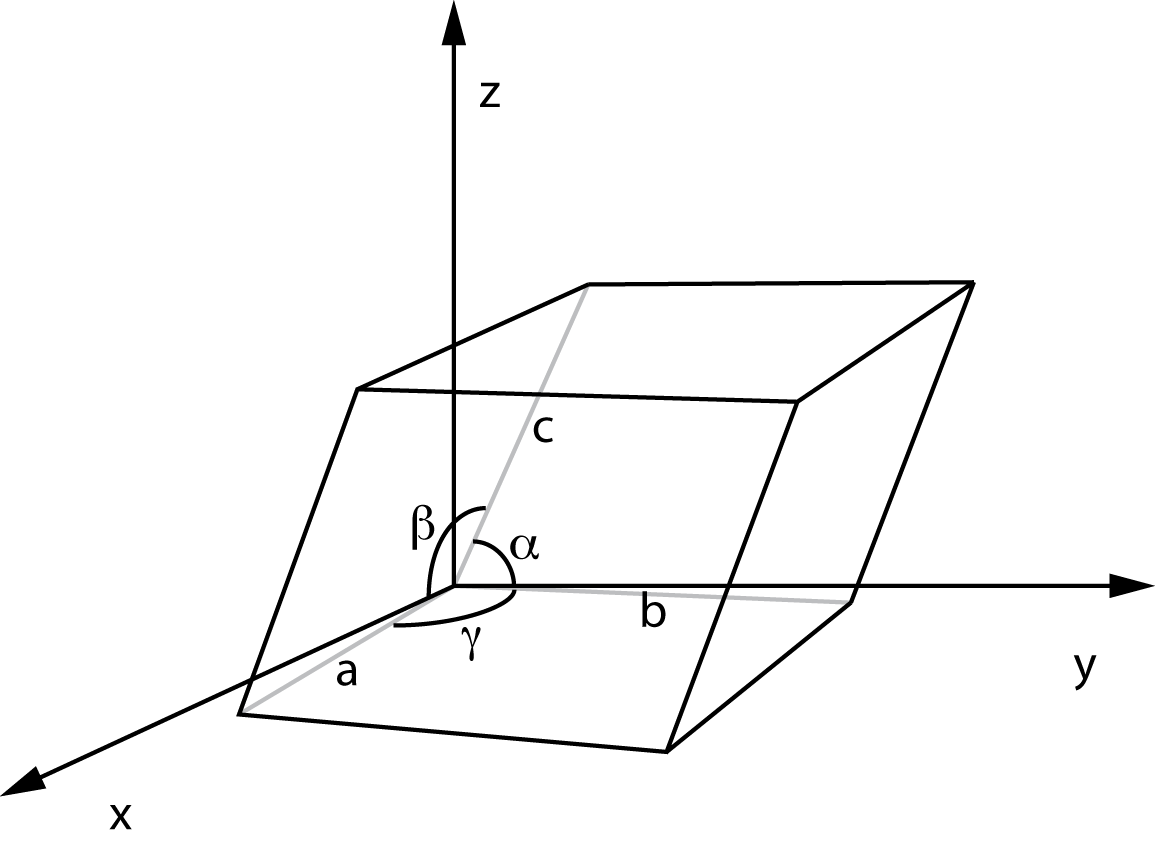
\includegraphics[width=.7\linewidth]{UnitCell.png}
\caption{A general unit cell with its six lattice constants}
\label{fig:unitcell}
\end{figure}

\cref{fig:unitcell} shows an example of unit cell randomly oriented in space. 
Although there are six parameters ($a,b,c, \alpha, \beta, \gamma$) available to describe the shape of the unit cell, the exact numerical representation of the unit cell, namely the base lattice vectors, is not easy to determine. 

To make the math a little bit easier, let assume that \vctr a is align with x-axis, which gives us
\[
	\vctr a = (a_1, a_2, a_3) = (a, 0, 0)
\]
Then let's determine the x-y plane through \vctr a and \vctr b.
In other words, \vctr b can be easily written out as
\[
	\vctr b = (b_1, b_2, b_3) = (b\cos\gamma, b\sin\gamma, 0)
\]
For a general unit cell, the volume of the cell is determined through its six lattice parameters/constants, 
\[
	V = abc\sqrt{1 + 2\cos\alpha\cos\beta\cos\gamma - \cos^2\alpha-\cos^2\beta-\cos^2\gamma}
\]
The volume of the unit cell can also be calculated through 
\[
	V = A_{xy}\cdot c_z = abc_3\sin\gamma 
\]
which gives us 
\[
	c_3 = \dfrac{V}{ab\sin\gamma}
\]
Arbitrary choice of the reference system should not affect the angle between two vectors, which gives us 

\begin{align*}
	\vctr a \cdot \vctr c &= ac\cos\beta   = a_1c_1 + a_2c_2 + a_3c_3 \\
	\vctr b \cdot \vctr c &= bc\cos\alpha = b_1c_1 + b_2c_2 + b_3c_3	
\end{align*}
Since \vctr a and \vctr b are known, we have
\begin{align*}
	a_1c_1 + 0 + 0 &= ac_1 = ac\cos\beta \\
	b_1c_1 + b_2c_2 + 0 &= bc_1\cos\gamma  + bc_2\sin\gamma  = bc\cos\alpha
\end{align*}
Solve the above linear system, we have
\begin{align*}
	c_1 &= c\cos\beta \\
	c_2 &= \dfrac{\cos\alpha - \cos\beta\cos\gamma}{\sin\gamma}c
\end{align*}
So the last base vector, \vctr c can be expressed as 
\[
	\vctr c = ( c \: \cos\beta, 
	                c \: \dfrac{\cos\alpha - \cos\beta\cos\gamma}{\sin\gamma}, 
	                \dfrac{V}{ab\sin\gamma})
\]
where $V$ is the volume of the unit cell.

To sum it up, for a general unit cell with six lattice parameters known, if we select \vctr a to be x-axis and \vctr b to lie in the x-y plane, the expression of base lattice vectors can be expressed as 
\begin{align*}
	\vctr a &= (a, 0, 0) \\
	\vctr b &= (b\cos\gamma, b\sin\gamma, 0) \\
	\vctr c &= ( c \: \cos\beta, 
	                c \: \dfrac{\cos\alpha - \cos\beta\cos\gamma}{\sin\gamma}, 
	                \dfrac{V}{ab\sin\gamma})
\end{align*}
where $V$ is the volume of the unit cell and can be calculate through
\[
	V = abc\sqrt{1 + 2\cos\alpha\cos\beta\cos\gamma - \cos^2\alpha-\cos^2\beta-\cos^2\gamma}.
\]

Another convection would be forcing \vctr b to be parallel to y-axis, however this convention has been dropped at APS.
Thus, there is no reason to consider other situation anymore.
\end{document}
